\documentclass[12pt,a4paper]{article}
\usepackage[utf8]{inputenc}
\usepackage[left=2.5cm,right=2.5cm,top=3cm,bottom=2cm]{geometry}
\author{Pauline Speckmann}
\usepackage{graphicx}

\usepackage{fancyhdr}
\pagestyle{fancy}
\fancyhf{}
\fancyhead[l]{Digitalisierung Vorlesung 2 $-$ Zusammenfassung von Pauline Speckmann}
\fancyhead[r]{\thepage}

\begin{document}
\setcounter{section}{1}
\section{Modellierung von Informationssystemen}


\vspace*{1cm}
\subsection{Modellbegriff und Modellierung} %%%%%%%%%%%%%%%%%%%%%%%%%%%%%%%%%%%%%%%%%%%%%%%%%%%%%%%%%%%%%%%%%%%%%%%%%%%%%%%%%%%%%
\begin{itemize}
   \item Nutzen von Modellen
      \begin{itemize}
         \item \textbf{Grundzweck}: Reduktion von Komplexität
         \item Modell ist stets Modell mit Gegenstand (wovon), Zweck (wozu) und Zielgruppe (für wen)
      \end{itemize}
      
   \item Merkmale: Verkürzungs-, pragmatisches und Abbildungsmerkmal
   
   \item Realität $\rightarrow$ IST-Modell $\rightarrow$ SOLL-Modell
      \begin{itemize}
         \item \textbf{IST-Modell}:  Abbild der realen Welt
         \item \textbf{SOLL-Modell}: Zukünftige Möglichkeiten
      \end{itemize}

   \item \textbf{Geschäftsprozessmodellierung}:
      \begin{itemize}
         \item Erhöhung der Transparenz von Prozessen und Beziehungen innerhalb eines Unternehmens
         \item Erkennen von Zusammenhängen in betrieblichen Abläufen
         \item Erklärung der Funktionsweise des Unternehmens
         \item Erleichterung der Kommunikation im Unternehmen
         \item Grundlage zur Prozessoptimierung
         \item Einsatz zur Darstellung und Analyse verschiedener Lösungen
      \end{itemize}

   \item \textbf{Referenzmodell}:
      \begin{itemize}
         \item Immaterielle Abbildung der verarbeiteten Informationen
         \item Besitzt (im Gegensatz zu einem normalen Modell) normativen Charakter (Gestaltungsempfehlungen) und Heterogenität
         \item Allgemeingültigkeitsanspruch (Wahl einer adäquaten Abstraktion)
         \item Flexibilität: Veränderungen mit geringem Aufwand durchführen
      \end{itemize}
\end{itemize}


\vspace*{0.5cm}
\subsection{Architektur integrierter Informationssysteme (ARIS)} %%%%%%%%%%%%%%%%%%%%%%%%%%%%%%%%%%%%%%%%%%%%%%%%%%%%%%%%%%%%%%%%
\begin{itemize}
   \item Architekturmodell zur Gestaltung einzelner Informationssysteme
          $\rightarrow$ Ausgangspunkt sind Vorgangskettenmodelle betrieblicher Bereiche
   \item ARIS umfasst:
      \begin{itemize}
        \item Vier Schichten: Daten (Zustände und Ereignisse), Funktionen, Steuerung und Organisation (inkludiert Bearbeiter)
        \item Drei Entwicklungsstufen
	        \begin{itemize}
	            \item[1)] Fachkonzept\\
	                  Ausgangspunkt für Umsetzung von Betriebswirtschaft in Informationstechnik
	                  (Anwendung einer formalisierten Sprache)
	            \item[2)] DV-Konzept (Datenverarbeitung)\\
	                  Übertragung der Begriffswelt von Fachkonzept in DV-Konzept und Definitionen
	            \item[3)] Implementierung\\
	                  Übergang des DV-Konzepts in Hard- und softwaretechnische Komponenten
	        \end{itemize}
      \end{itemize}
\end{itemize}


\vspace*{0.5cm}
\subsection{Modellierung von Geschäftsprozessen} %%%%%%%%%%%%%%%%%%%%%%%%%%%%%%%%%%%%%%%%%%%%%%%%%%%%%%%%%%%%%%%%%%%%%%%%%%%%%%%%
\begin{itemize}
   \item \textbf{Ereignisgesteuerte Prozessketten (EPK)}:
       \begin{itemize}
		   \item Startereignis \& Endereignis
		   \item Modellierungselemente Ereignis \& Funktion
		   \item Operatoren AND, OR, XOR
		\end{itemize}
\end{itemize}

\vspace*{-0.8cm}
\begin{center}
    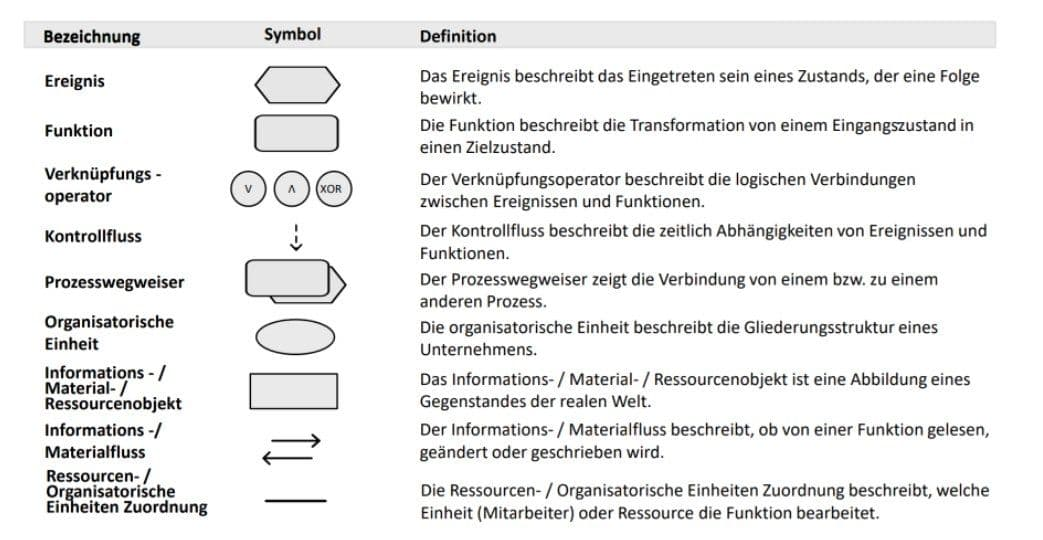
\includegraphics[width=1.05\textwidth]{digi2.jpg}
\end{center}

\begin{itemize}
\item []
   \begin{itemize}
      \item EPK braucht min. 1 Startereignis (oder Prozessschnittstelle)
	   \item EPK braucht min. 1 Endereignis (oder Prozessschnittstelle)
	   \item Auf Ereignis folgt Funktion oder Konnektor (Ausnahme: Endereignis)
	   \item Auf Funktion folgt Ereignis oder Konnektor
	   \item Jede Funktion hat genau eine ausgehende Kante
	   \item Jedes Ereignis hat genau eine eingehende und eine ausgehende Kante (Ausnahme: Start- und Endereignis)
	   \item Konnektor hat \textit{entweder} mehrere eingehende und genau eine ausgehende Kante 
	         \textit{oder} genau eine eingehende und mehrere ausgehende Kanten
   \end{itemize}
\end{itemize}


\vspace*{0.5cm}
\subsection{Analyse von Geschäftsprozessen mit Process-Mining} %%%%%%%%%%%%%%%%%%%%%%%%%%%%%%%%%%%%%%%%%%%%%%%%%%%%%%%%%%%%%%%%%%
\begin{itemize}
   \item \textbf{$\alpha$-Algorithmus}:
      \begin{itemize}
         \item Grundidee:\\
               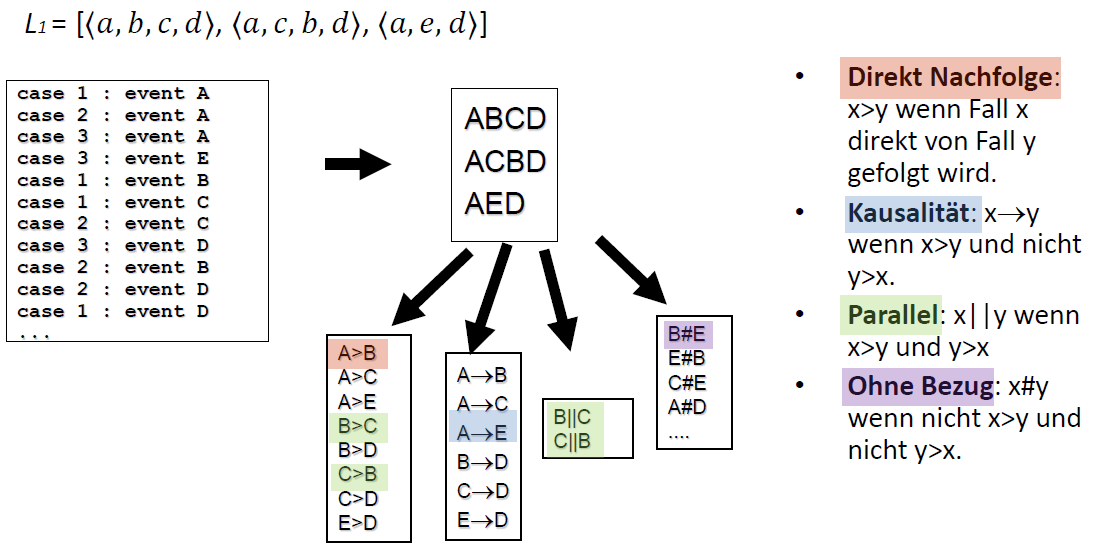
\includegraphics[width=0.9\textwidth]{alphaAlgorithmusGrundidee.png}
         \item Übersetzung ins finale Prozessmodell\\
               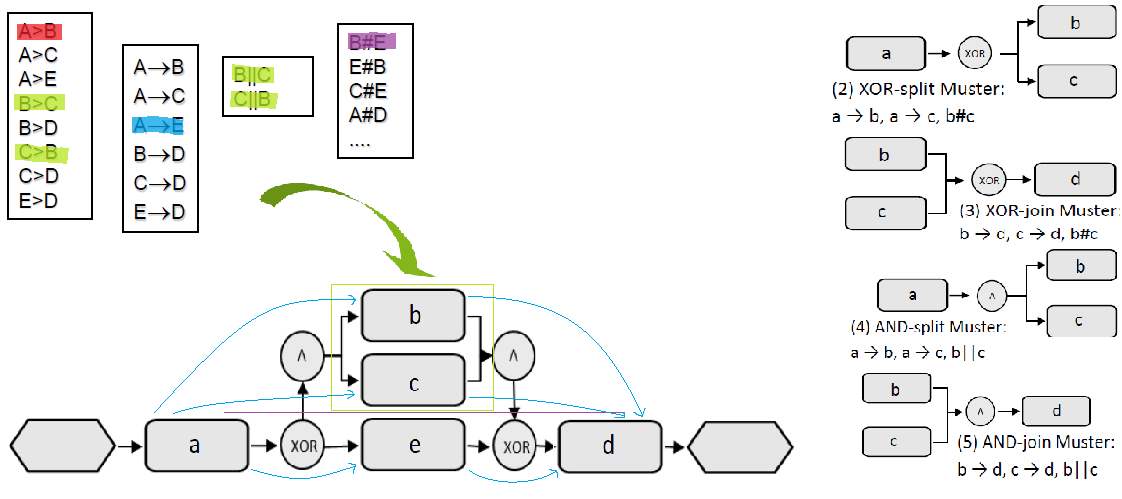
\includegraphics[width=0.9\textwidth]{alphaAlgFinalesModell.png}
      \end{itemize}
\end{itemize}

\end{document}